% ECIR 2027 -- SHORT PAPER, FIRST DRAFT
%
% Prepared with the official Springer LNCS template (llncs.cls v2.25, 2026/09/03) supplied with
% the call, and checked against "Instructions for Authors of Papers to be Published in Springer
% Computer Science Proceedings". Compliance notes:
%   Sec. 4.2  short papers are 6-11 pages; this draft is inside that range with Secs. 1 and 6
%             still to be written.
%   Sec. 4.5  no colour is used in text, tables or equations; both figures are greyscale with
%             distinct markers/hatching so they survive black-and-white printing, are vector
%             PDFs, and are drawn at the true text width so no label falls below 6 pt.
%   Sec. 4.1  only two heading levels are numbered; propositions are numbered consecutively
%             with no section counter, using the class's own environment (no self-defined ones).
%   Sec. 4.9  citations by number via splncs04.
%
% LOCAL BUILD NOTE: newtxtext/newtxmath are not installed on the machine this was drafted on, so
% local compilation used the CMR fallback (comment the two newtx lines to reproduce that). The
% lines are kept because the supplied template specifies them; build on Overleaf or any TeX Live
% with newtx for the submission PDF.
%
% STATUS: Sec. 1 (Introduction) and Sec. 6 (Related Work) are deliberate stubs.
%
\documentclass[runningheads]{llncs}

\usepackage[T1]{fontenc}
\usepackage{newtxtext}
\usepackage[varvw]{newtxmath}
\usepackage{graphicx}
\usepackage{booktabs}
\usepackage{amsmath}

\newcommand{\NE}{\mathrm{NE}}
\newcommand{\ind}{\mathbf{1}}   % avoids depending on amssymb/newtxmath for \mathbb

\begin{document}

\title{How Much of the Delayed-Feedback Penalty Is Recoverable?}
\titlerunning{How Much of the Delayed-Feedback Penalty Is Recoverable?}

\author{Anonymous Author\inst{1}}
\authorrunning{A. Author}
\institute{Anonymous Institution, Anonymous City, Country\\
\email{anonymous@example.org}}

\maketitle

\begin{abstract}
Conversion labels arrive late, so a model trained today must either wait for labels and train on
stale data, or use fresh data whose labels are only partly observed. We derive a closed-form
ceiling on how much of the resulting loss a censoring-corrected estimator can recover: it is the
mean relative Fisher information of the censored observations, computable from the empirical
delay distribution alone, before any model is trained. On the Criteo delayed-feedback corpus that
ceiling is $0.868$ for a seven-day attribution window. We test it with 1{,}600 runs spanning five
model capacities, twenty rolling origins and five delayed-label strategies under one protocol.
Censoring correction attains $0.883$, $0.874$ and $0.849$ of the penalty at the three smallest
capacities, within $0.02$ of the predicted ceiling, then falls to $0.625$ at the largest. We show
the shortfall is misspecification rather than estimation error: the delay distribution varies
sharply with the covariates, and only a model expressive enough to resolve that variation is
harmed by assuming it away. We further show that the apparent advantage of knowledge distillation
here is mostly capacity transfer rather than delay mitigation, and give the control that separates
the two.

\keywords{Delayed feedback \and Conversion rate prediction \and Censored labels \and Knowledge
distillation \and Computational advertising}
\end{abstract}

\section{Introduction}

\emph{[To be written. Contribution bullets to land here: (i)~a parameter-free ceiling on
recoverable delayed-feedback loss, validated to within $0.02$; (ii)~the capacity regime in which
censoring correction saturates that ceiling and the regime in which it does not, with the measured
cause; (iii)~a control separating distillation's capacity transfer from genuine delay
mitigation.]}

\section{Problem Setting}
\label{sec:setting}

A click occurs at time $t$ with covariates $x$. If it converts, the conversion follows after a
delay $d>0$; write $d=\infty$ for a click that never converts. Under an attribution window
$\Delta$ the prediction target is
\begin{equation}
y \;=\; \ind[d \le \Delta], \qquad \eta(x) \;=\; \Pr(d \le \Delta \mid x).
\label{eq:label}
\end{equation}

The difficulty is not that $y$ is noisy but that it is not yet determined. At an origin $T$, the
moment a training set is assembled, a row clicked at $t$ has been observable for
\begin{equation}
e(t) \;=\; \mathrm{clip}(T-t,\;0,\;\Delta),
\qquad
y_{\mathrm{obs}} \;=\; \ind[d \le e(t)] \;\le\; y .
\label{eq:obs}
\end{equation}
Two regimes follow. If $t \le T-\Delta$ then $e=\Delta$ and $y_{\mathrm{obs}}=y$ exactly. If
$t > T-\Delta$ the row is right-censored: $y_{\mathrm{obs}}=1$ is conclusive, but
$y_{\mathrm{obs}}=0$ is ambiguous, because the click may still convert inside its remaining
window. Everything below follows from \eqref{eq:obs}, and no strategy is granted an assumption
the others lack.

\subsection{Five Strategies as Estimators}

Let $\mathcal{M}=[0,T-\Delta)$ denote the mature rows and $\mathcal{C}=[T-\Delta,T)$ the censored
ones, with $|\mathcal{M}|=m$ and $|\mathcal{C}|=c$. Table~\ref{tab:arms} states each strategy as a
choice of training set and target. The oracle is infeasible at time $T$, since it uses labels that
do not yet exist; it serves only as the denominator for how much of the penalty a feasible
strategy recovers.

\begin{table}[t]
\caption{The five strategies, with the infeasible oracle and the distillation control. All are
evaluated on the same held-out day against the same target \eqref{eq:label}}
\label{tab:arms}
\centering
\begin{tabular}{@{}llp{5.1cm}@{}}
\toprule
& training set & target \\
\midrule
Oracle & $\mathcal{M}\cup\mathcal{C}$ & true $y$ (infeasible at $T$) \\
A, wait & $\mathcal{M}$ & $y$ \\
B, distil & $\mathcal{M}\cup\mathcal{C}$ & teacher's $\hat\eta$; teacher trained on $\mathcal{M}$ \\
B$^-$, control & $\mathcal{M}$ & the same teacher's $\hat\eta$ \\
C, correct & $\mathcal{M}\cup\mathcal{C}$ & $y_{\mathrm{obs}}$; loss on $\sigma(z)\hat F(e)$, serve $\sigma(z)$ \\
D, band & $[0,T-u_k)$, $k=1\ldots K$ & $\ind[u_{k-1}<d\le u_k]$, predictions summed \\
E, reweight & $\mathcal{M}$ & $y$, weighted by $\hat p_{\mathcal{C}}(x)/\hat p_{\mathcal{M}}(x)$ \\
\bottomrule
\end{tabular}
\end{table}

Strategy C is the classical joint conversion-delay likelihood \cite{chapelle2014modeling} with a
non-parametric $\hat F$. Under the conditional-independence assumption
\begin{equation}
\Pr(d \le e \mid x,\ d \le \Delta) \;=\; F(e),
\label{eq:a1}
\end{equation}
that is, delay independent of the covariates given conversion inside the window, the observed
label has mean $\Pr(y_{\mathrm{obs}}=1 \mid x,e)=\eta(x)F(e)$. Fitting $\sigma(z(x))\hat F(e)$
against $y_{\mathrm{obs}}$ under log loss is then a proper composite likelihood for $\eta$. The
correction lives in the loss, and $\sigma(z)$ is served directly with no post-hoc rescaling.

B$^-$ is not an ablation but a necessary control. Strategy B changes two things at once relative
to A: the student inherits a teacher that may be larger than itself, and it trains on covariates
that A had to discard. B$^-$ removes only the second. Without it, any gain from B is
unattributable.

\section{How Much Is Recoverable?}
\label{sec:theory}

We now bound what any estimator of the form C can recover, using only the delay distribution.

Under \eqref{eq:a1} a censored observation with window $e$ is Bernoulli with mean $\eta F(e)$. Its
Fisher information about $\eta$ is $I(\eta;e)=(\partial_\eta \eta F)^2/(\eta F(1-\eta F))
= F/(\eta(1-\eta F))$, against $I_{\mathrm{full}}=1/(\eta(1-\eta))$ for a mature row. The relative
information of a censored row is therefore
\begin{equation}
\rho(F) \;=\; \frac{I(\eta;e)}{I_{\mathrm{full}}} \;=\; \frac{F(1-\eta)}{1-\eta F} \;\in\; [0,1],
\qquad \rho(1)=1, \quad \rho(F)\approx F \ \text{for small } \eta .
\label{eq:rho}
\end{equation}

\begin{proposition}
\label{prop:ceiling}
Assume \eqref{eq:a1}, and that excess risk scales as $1/n$ in the effective sample size. Let
$\bar\rho = |\mathcal{C}|^{-1}\sum_{i\in\mathcal{C}}\rho(F(e_i))$. Then the fraction of the
oracle-minus-wait gap recovered by strategy C is
\begin{equation}
R \;=\; \frac{1/m - 1/(m+\bar\rho c)}{1/m - 1/(m+c)} \;=\; \frac{\bar\rho\,(m+c)}{m+\bar\rho c}.
\label{eq:recovery}
\end{equation}
\end{proposition}

$R$ contains no fitted quantity: $\bar\rho$ follows from the empirical delay distribution and the
base rate, and $m$ and $c$ from the calendar. It can be computed before training anything.

On this corpus the delay distribution is strongly front-loaded, with $57.4\,\%$ of conversions
within seven days landing in the first hour, so censored rows retain most of their information
even when their window has barely opened. Averaged over the twenty origins used below,
$\bar\rho=0.886$ and $R=0.888$ for $\Delta=1$\,d, and $\bar\rho=0.847$ and $R=0.868$ for
$\Delta=7$\,d.

Proposition~\ref{prop:ceiling} prices the statistical cost of censoring only. It assumes
\eqref{eq:a1} holds, and it attributes the whole oracle-minus-wait gap to effective sample size,
ignoring covariate shift between $\mathcal{M}$ and the served day. Section~\ref{sec:results} shows
both idealisations are visible in the data, and identifies which one binds.

\section{Experimental Design}
\label{sec:design}

\paragraph{Protocol.}
We use rolling origins $T=40,\ldots,59$, each with training windows ending at $T$ minus that
strategy's own wait, and evaluation on the single day $[(T{+}1)\mathrm{d},(T{+}2)\mathrm{d})$ with
one idle day in between, held fixed as the window slides. The label \eqref{eq:label} is enforced
identically in training and evaluation: a row may enter a training set only if its label is
knowable at $T$. Evaluation days carry 230k to 300k rows. Conversions are logged to day $90.955$
while clicks stop at day $61.001$, so every evaluation label is fully resolved at every $\Delta$.
The origin is the unit of replication and all comparisons are paired on it, because the evaluation
positive rate swings from $0.1595$ to $0.1966$ across these twenty days, an order of magnitude
more than any effect we measure.

\paragraph{Tasks.}
We use $\Delta\in\{1\mathrm{d},7\mathrm{d}\}$ and drop $\Delta=1$\,h, whose oracle gap is
$-0.00002$ ($p=0.842$): there is no penalty to recover, so every strategy ties with A by
construction.

\paragraph{Capacity Ladder.}
Strategy rankings that hold at one model size need not hold at another, so the entire comparison
is repeated at five capacities $S_0,\ldots,S_4$. All five share one backbone and differ only in
the number of categorical hash-table rows, a single monotone knob that is exactly the
embedding-table memory footprint, which is the binding constraint in production ranking. The five
are approximately equally spaced in normalised entropy by construction (mean step $0.0149$;
Table~\ref{tab:ladder}) and are monotone in it at 40 of 40 (task, origin) cells.

\begin{table}[t]
\caption{The capacity ladder. Table parameters vary over $3{,}641\times$ and the resulting
normalised entropy is approximately equally spaced}
\label{tab:ladder}
\centering
\begin{tabular}{@{}lrrrrr@{}}
\toprule
& $S_0$ & $S_1$ & $S_2$ & $S_3$ & $S_4$ \\
\midrule
hash rows & 36 & 64 & 160 & 896 & 131{,}072 \\
table parameters & 2{,}592 & 4{,}608 & 11{,}520 & 64{,}512 & 9{,}437{,}184 \\
$\NE$ ($\Delta{=}7$d, one origin) & 0.78626 & 0.77312 & 0.75730 & 0.74124 & 0.72794 \\
\bottomrule
\end{tabular}
\end{table}

\paragraph{Teacher.}
Strategy B always uses the same teacher, selected as the best of a 21-rung architecture ladder and
held at full table resolution. The teacher sees A's window and A's labels, so it differs from A on
capacity alone, receiving no extra data and no extra label information.

\paragraph{Metrics.}
We report normalised entropy $\NE=\text{logloss}/H(\bar y)$, the calibration ratio $\bar p/\bar y$,
and a calibration-adjusted $\NE$ obtained by multiplying every prediction by $c=\bar y/\bar p$, so
that calibration is exactly one, and recomputing $\NE$. That quantity can exceed $\NE$, because
matching the mean is not the same as minimising log loss; it is a level-matching diagnostic, not a
lower bound. All models train for exactly one epoch: a second epoch already overfits at every
capacity (train $-0.0186$, evaluation $+0.0019$, $p=0.025$).

\paragraph{Scale and Verification.}
The grid is 2 tasks $\times$ 5 capacities $\times$ 20 origins $\times$ 8 arms, or 1{,}600 scored
runs. Before launching we verified that the calibration multiplier forces calibration to one at
every starting bias; that the harness reproduces previously logged cells bit-exactly (14 of 14,
absolute difference $0$); that the shared teacher is identical across capacities to seven decimal
places while student models are not; and that every arm at a given (task, origin) is scored on an
identical evaluation set.

\section{Results}
\label{sec:results}

\subsection{The Penalty Depends on the Window, Not Much on Capacity}

The oracle-minus-wait gap at $\Delta=7$\,d is $+0.00538$, $+0.00602$, $+0.00746$, $+0.00842$ and
$+0.00598$ for $S_0$ through $S_4$, all with $p<0.001$ over 20 of 20 origins. At $\Delta=1$\,d it
is an order of magnitude smaller, from $+0.00067$ to $+0.00092$. Waiting is expensive only when
the window is long relative to the available history: at seven days it withholds $12.6$ to
$18.6\,\%$ of the corpus.

\subsection{The Ceiling Is Attained, and Then It Is Not}

\begin{figure}[t]
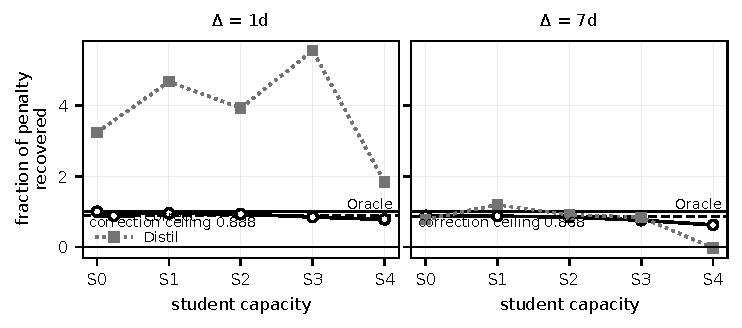
\includegraphics[width=\textwidth]{figs/fig1_recovery.pdf}
\caption{Measured recovery of the delay penalty against the parameter-free ceiling of
Proposition~\ref{prop:ceiling} (dashed). Censoring correction (C, open circles) tracks the ceiling
at the three smallest capacities and falls away at the two largest. Distillation (B, grey squares)
behaves differently and exceeds one at $S_1$ for $\Delta=7$d, because the oracle is capped at the
student's capacity whereas the teacher is not}
\label{fig:recovery}
\end{figure}

Figure~\ref{fig:recovery} is the central result. For $\Delta=7$\,d the predicted ceiling is
$0.868$, and C measures $0.883$, $0.874$, $0.849$, $0.759$ and $0.625$ across $S_0$ through $S_4$.
At the three smallest capacities the prediction is accurate to $+0.015$, $+0.006$ and $-0.019$,
from a formula with no free parameters that was fitted to nothing. At $S_3$ and $S_4$ it
over-predicts by $0.11$ and $0.24$.

\subsection{The Shortfall Is Misspecification, Not Estimation}

Proposition~\ref{prop:ceiling} assumes \eqref{eq:a1}, and that assumption is false on this corpus
in a way we can measure. Stratifying converted rows by the distinct values of a single categorical
field, the share of within-seven-day conversions landing in the first hour ranges from $0.453$ to
$0.689$, and the median delay from $0.16$\,h to $1.73$\,h, a tenfold spread
(Table~\ref{tab:strata}).

\begin{table}[t]
\caption{The delay distribution is strongly covariate-dependent, violating \eqref{eq:a1}. Strata
are distinct values of one categorical field; the pooled $F(1\mathrm{h})$ is $0.574$}
\label{tab:strata}
\centering
\begin{tabular}{@{}lrrrrrr@{}}
\toprule
stratum & 1 & 2 & 3 & 4 & 5 & 6 \\
\midrule
conversions $\le 7$d & 860{,}851 & 441{,}893 & 434{,}540 & 192{,}949 & 134{,}479 & 23{,}790 \\
$F(1\mathrm{h})$ & 0.453 & 0.576 & 0.602 & 0.628 & 0.689 & 0.687 \\
median delay (h) & 1.73 & 0.41 & 0.29 & 0.34 & 0.23 & 0.23 \\
\bottomrule
\end{tabular}
\end{table}

This resolves the pattern in Fig.~\ref{fig:recovery}. A model too small to resolve
covariate-dependent delay cannot be harmed by a correction that assumes it away, so at $S_0$
through $S_2$ the only cost of censoring is the statistical one that
Proposition~\ref{prop:ceiling} prices exactly. As capacity grows, the misspecification bias in
$\hat F(e)$ becomes expressible and recovery falls below the ceiling. The prediction is therefore
best read as an upper bound that is tight precisely when the model is sample-limited rather than
bias-limited, and the gap between prediction and measurement estimates what a
covariate-conditional delay model would buy.

\subsection{Distillation's Advantage Is Mostly Not About Delay}

\begin{figure}[t]
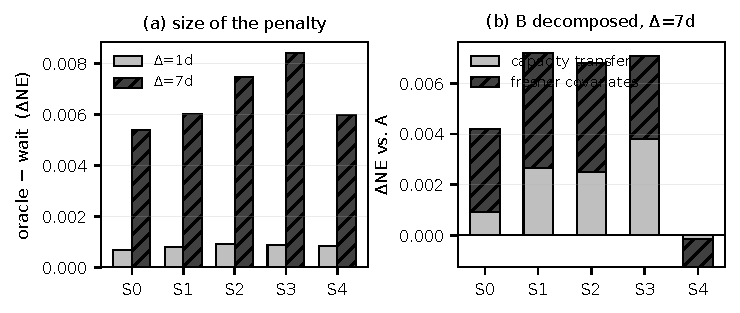
\includegraphics[width=\textwidth]{figs/fig2_penalty_decomp.pdf}
\caption{(a)~The delay penalty by capacity and window. (b)~Strategy B decomposed using the B$^-$
control into capacity transfer and exposure to fresher covariates. At $\Delta=7$d the
fresh-covariate term is $47$ to $78\,\%$ of the gain; at $\Delta=1$d, where little penalty exists
to recover, it is $6$ to $29\,\%$}
\label{fig:decomp}
\end{figure}

Strategy B beats A at $\Delta=7$\,d by $+0.00419$ to $+0.00722$ for $S_0$ through $S_3$, all with
$p \le 0.001$ over 19 of 20 origins. Read alone this looks like delay mitigation. The B$^-$ control
shows it is largely not: capacity transfer accounts for $22$ to $53\,\%$ of the gain at
$\Delta=7$\,d across $S_0$ through $S_3$, and $71$ to $94\,\%$ at $\Delta=1$\,d
(Fig.~\ref{fig:decomp}b). Only the residual, the student's exposure to covariates that A discarded
and which carry no new label information, is attributable to the delayed label; it is significant
at every capacity ($p \le 0.001$) but never dominant at the short window. At $S_4$, where the
teacher's headroom over the student is only $+0.0036$, B collapses to $-0.00015$ ($p=0.898$):
distillation helps exactly while the teacher is meaningfully better than the student, which is a
statement about model size rather than about feedback delay.

Strategies D and E do not repay their complexity. D ranges from $-0.00215$ to $+0.00457$ with no
monotone pattern in capacity; its slowest band still trains on A's window and so never escapes the
wait it was designed to avoid. E stays within $\pm 0.0027$ of A everywhere, consistent with the
penalty being missing labels rather than covariate staleness, and E by construction never touches
an unresolved label.

\section{Related Work}

\emph{[To be written. Anchor on the joint conversion-delay likelihood \cite{chapelle2014modeling};
the importance-weighting line \cite{ktena2019addressing,yasui2020feedback,yang2021capturing};
stream-level alternatives \cite{gu2021real,chen2022asymptotically}; and covariate-conditional
delay \cite{yang2022generalized,zhao2023escdfm}, which targets exactly the assumption
Section~\ref{sec:results} shows is violated.]}

\section{Limitations}

We use one seed per origin. The origin is the unit of replication ($n=20$), and seed sensitivity
was characterised separately at a standard deviation of $0.0004$ to $0.0030$, an order of
magnitude below the $\Delta=7$\,d effects, but seeds are not averaged here. The twenty origins
share training data heavily, so the effective sample size is below twenty.
Proposition~\ref{prop:ceiling} assumes a $1/n$ excess-risk rate, which we do not verify directly;
its empirical accuracy at $S_0$ through $S_2$ is the evidence offered. The calibration multiplier
is fitted on evaluation labels and is a diagnostic, never an achievable score. Strategy B's soft
targets are largely teacher in-sample on $\mathcal{M}$, and out-of-fold targets, the standard
remedy, are untested. Finally, all results come from a single public corpus with one delay
distribution; the ceiling is corpus-specific even though the formula is not.

\begin{credits}
\subsubsection{\ackname} \emph{[To be added after review.]}

\subsubsection{\discintname}
The authors have no competing interests to declare that are relevant to the content of this
article.
\end{credits}

\bibliographystyle{splncs04}
\bibliography{refs}

\end{document}
